\noindent\textbf{1.} Như được chỉ ra trên hình 4.1, góc vì $\sin\alpha=\dfrac{1}{2}$ nên $\alpha=30^\circ$. Theo định luật khúc xạ ánh sáng
\begin{equation*}
  \sin\beta=\frac{\sin\alpha}{n}=\frac{1}{2n}\Rightarrow\tan\beta=\frac{1}{\sqrt{4n^{2}-1}}
\end{equation*}
từ hình vẽ, dễ dàng nhận thấy
\begin{equation*}
  \begin{gathered}
    x_{0}=\frac{R}{2}-\frac{\sqrt{3}}{2}R\tan\gamma \\
    \tan\gamma=\tan(\alpha-\beta)=\frac{\tan\alpha-\tan\beta}{1+\tan\alpha\tan\beta}=\frac{\sqrt{4n^{2}-1}-\sqrt{3}}{\sqrt{12n^{2}-3}+1} \\
    x_{0}=\frac{R}{2}\left(1-\frac{\sqrt{12n^{2}-3}-3}{\sqrt{12n^{2}-3}+1}\right)=\frac{2R}{\sqrt{12n^{2}-3}+1}
  \end{gathered}
\end{equation*}

\noindent\textbf{2.} Tại thời điểm $t$, mặt tiếp xúc sẽ có dạng một hình tròn bán kính $r$. Trong thời gian $dt$ tiếp theo, nhiệt lượng truyền vào khối băng là
\begin{equation*}
  \mathrm{d}Q=K\pi r^{2}dt
\end{equation*}
với $K$ là hằng số. Thể tích băng nóng chảy là
\begin{equation*}
  dQ=Ldm=L\rho\pi r^{2}dz
\end{equation*}
với $L$ và $\rho$ tương ứng là ẩn nhiệt chuyển pha và khối lượng riêng của băng. Như vậy ta có
\begin{equation*}
  K\pi r^{2}dt=-L\rho\pi r^{2}dz
\end{equation*}
\begin{equation*}
  \Rightarrow\frac{dz}{dt}=-\frac{K}{L\rho}=\text{const}
\end{equation*}
do đó
\begin{equation*}
  z(t)=R\left(1-\frac{t}{T_0}\right)
\end{equation*}

\begin{figure}[h]
  \centering
  \begin{subfigure}[b]{0.49\textwidth}
    \centering
    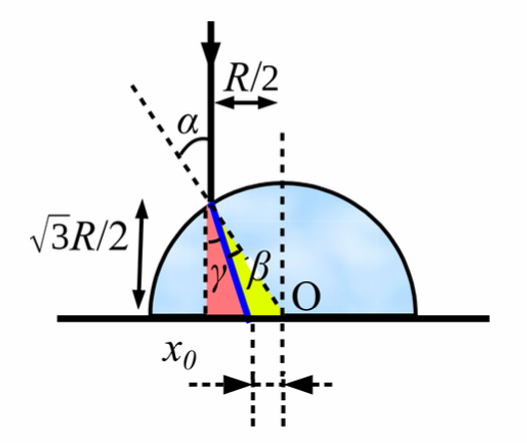
\includegraphics[width=0.95\textwidth]{Figures/Solutions/Fig 4.1.png}
    \begin{center}
      \figurename{ 4.1}
    \end{center}
  \end{subfigure}
  \hfill
  \begin{subfigure}[b]{0.49\textwidth}
    \centering
    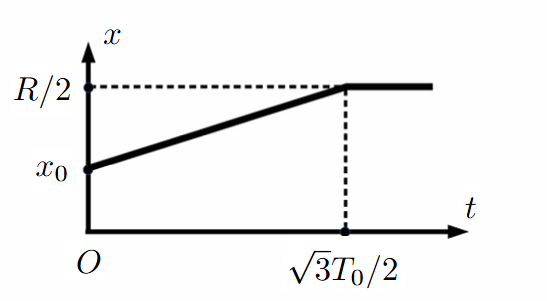
\includegraphics[width=0.95\textwidth]{Figures/Solutions/Fig 4.2.png}
    \begin{center}
      \figurename{ 4.2}
    \end{center}
  \end{subfigure}
\end{figure}

\noindent\textbf{3.} Khi bán kính của khối băng nhỏ hơn hoặc bằng $\dfrac{R}{2}$, chùm laser sẽ chiếu thẳng xuống bàn, tức $x(t)=\dfrac{R}{2}$. Khi này độ cao của khối băng là $z(t)=\left(1-\frac{\sqrt{3}}{2}\right)R$, điều này sẽ xảy ra tại $t=\dfrac{\sqrt{3}}{2}T_0$. Như vậy, với $t>\dfrac{\sqrt{3}}{2}T_0$, ta có $x(t)=\dfrac{R}{2}$.\\
\noindent Với $t<\dfrac{\sqrt{3}}{2}T_0$, ta sẽ sử dụng các tam giác đồng dạng
\begin{equation*}
  \begin{gathered}
    \frac{\frac{R}{2}-x_{0}}{\frac{R}{2}-x(t)}=\frac{\frac{\sqrt{3}}{2}R}{R\left(\frac{\sqrt{3}}{2}-\frac{t}{T_{0}}\right)} \\
    \Rightarrow\left(\frac{R}{2}-x_{0}\right)\left(\frac{\sqrt{3}}{2}-\frac{t}{T_{0}}\right)=\frac{\sqrt{3}}{2}\left(\frac{R}{2}-x\right) \\
    \Rightarrow x(t)=\frac{R}{2}-\left(\frac{R}{2}-x_{0}\right)\left(1-\frac{2}{\sqrt{3}}\frac{t}{T_{0}}\right)=\frac{R}{2}-\frac{R}{2}\left(1-\frac{4}{\sqrt{12n^{2}-3}+1}\right)\left(1-\frac{2}{\sqrt{3}}\frac{t}{T_{0}}\right)
  \end{gathered}
\end{equation*}